\chapter{Introduction}
With the maturity of database technologies, nowadays
applications collect data in all domains at an
unprecedented scale. For example, billions of 
social network users and their activities are collected in the form
of \emph{graphs}; Thousand sensor reports are collected per second
in the form of \emph{time series}; Hundreds of millions of temporal-locations
are collected as \emph{trajectories}, to name just a few. Flooded by the
tremendous amount of data, it is emerging to 
provide useful and efficient analytics for various data domains.
Traditional SQL-based analytics which comprises 
of primitives (such as, partition, sorting and aggregation etc.)
become limited in non-structured domains.
In SQL context, interesting analytics such as graph traversal and pattern detection
often involve complex joins which are very hard to optimize 
without domain knowledge.
In this thesis, we explore the neighborhood data analytic, which
in SQL is expressed by the window function,
on different domains and demonstrate how to efficiently deploy
neighborhood data analytic to gain useful data insights.
%
%Traditional SQL-based analytics including ranking, aggregation, 
%and window functions, has seen a great success in supporting
%data-based decision-makings on relational data. However, 
%when applying SQL-based analytics on other data domains, it often
%involves expensive joins which are hard to optimize without leveraging the domain
%knowledge. For instance, when computing the $K$-hop neighborhoods of vertexes in a graph, 
%SQL-based traversal of graph involves multi-rounds of joins, which is inefficient
%than search-based traversal~\cite{}. Or, when searching for a group of objects
%that travels together for a certain time, SQL-based solution would involves
%recursive joins and chain joins.
%
%See from the limitation of SQL-analytic on those domains, in this thesis, we 
%explore the neighborhood based analytics in various data domains.
%In particular, we address three issues. First, we define the neighborhoods
%on various domains. Second, we showcase the usefulness of neighborhood analytics 
%on data models.
%Third, we address the efficiency issues on applying the neighborhood
%analytics in different data domains for large data.

% 
%With the rapid advancement of technologies, 
%many applications nowadays generate floods of data. 
%For example, social network users and their
%activities generate graph data; News events generate
%streams of texts; and moving vehicles generate spatial-temporal trajectories.
%These data embeds a wealth of information from different domains 
%which is crucial in supporting data-driven decision-makings. An 
%important tasks in management of these data is to provide useful analytics
%to facilitate the discovery of data insights. Thus, the design of 
%effective methods for data analysis under different application domains 
%has drawn a tremendous attention from both industries and academia recently.
%
%Traditional SQL-defined analytics which are specifically designed for
%structured data faces two major issues in supporting data analytics under
%various domains. First, SQL analytics has limited operations which may not
%be suitable for some applications. Second, SQL analytics may loose semantic
%meaning in no-structured or semi-structured data.

%Traditionally,  SQL-defined analytics becomes limited when handling data with such heterogeneity.
%Opposed to the one-set-fits-all SQL analytics,
%ad-hoc analytics for each domain are often required.
% Thus, the design
%of 
%
%An important aspect in data analytics is to study the data objects
%that are locally connected, as these data demonstrates strong clustering features. Such a kind 
%of analytic is referred as \emph{neighborhood analytic}. Nevertheless, the neighborhood
%analytic is prevalently seen in many area of applications.


 
%
%nowadays data are collected 
%at unprecedented scale. With the heterogeneity of data, many
%decisions that are painstakingly constructed manually 
%increasingly rely on data insights. 
%A crucial taks in management of such data is to provide useful analytics to 
%With the whole suite of the SQL analytic tools, data-driven decisions are 
%
%Decisions that previously were based on guesswork, or on	
%painstakingly constructed models of reality, can now be made based on the data itself. 
%A crucial task in management of data is to provide useful
%analytics to facilitate the discovery of data insights.
%
%As we
%enter the era of ``Big-data'', traditional SQL 
%analytics, which are designed specifically for structural relational data,
%are becoming shorthanded in supporting data with heterogeneity. 
%
%We are awash in	a flood of data today.	 In	 a broad range of application areas, data is being	
%collected at unprecedented scale.	 	 Decisions that previously were based	 on guesswork, or	 on	
%painstakingly constructed models of reality, can now be made based on the data itself.	 Such Big Data	
%analysis now drives nearly every aspect of our	 modern society, including mobile services, retail,	
%manufacturing, financial	services, life sciences, and	physical	sciences.
%
%``Big-data'', famous for its heterogeneity, scale and complexity, 
%has entering to the research horizon with promising potential 
%in data-driven decision-making. There has been an increasing needs
%for analyzing, understanding and processing ``big-data'' from
%both industrial and academic perspective. 
%
%``Neighborhood'' based analytic has been a complementary method
%for analyze data from a local perspective, which plays an important
%role in traditional data analytics. For instance, density-based spatial
%clustering examines the ....  egocentric network analysis,  SQL window
%function... Semi-Lazy data mining,
%to name a few. While these analytics are successful in 
%traditional area, it is left unknown whether ``neighborhood'' 
%based analytic is able to discover more insights in Big-data era.
%
%
%As being part of the research efforts
%in closing the gap between the potential of ``big-data'' and its realization,
%this thesis investigates the possibility of introducing ``neighborhood''-based
%analytic to ``big-data'' analysis. Specifically, we propose and analyze
% ``neighborhood''-based analytic in three heterogeneous domains: graph data,
% stream data, and spatial-temporal data. We design ad-hoc ``neighborhood''
% based data analytic on each data domain, and demonstrate the effectiveness
% of these analytic. We further address the challenges of applying these
% analytic efficiently by designing efficient index, powerful pruning, and scalable systems.
%
%
%The promise	of data-driven decision-making is now being recognized broadly, 
%and there is growing enthusiasm for	the notion of ``Big Data''.	 
%While the promise of Big Data is real -- for example, it is 
%estimated that Google alone contributed	54 billion dollars to the US economy
%in 2009 -- there is	currently a wide gap between its potential and its realization.
%Heterogeneity, scale, timeliness, complexity, and	privacy	 problems
%with Big Data impede progress at all phases of the pipeline that can create value from data.
%The problems start right away during data acquisition, when the data tsunami requires us to make decisions, currently in an ad hoc	manner, about what data to keep and what to discard, and how to store what	we keep reliably	with the	
%right metadata.	 Much data today is not natively in structured format; for example, tweets	and blogs are	
%weakly structured pieces of text,	while images and video are structured for storage and display, but not	
%for semantic content and search: transforming such content into a structured format for later analysis is	
%a major challenge. The value of data explodes when it can be linked with other data, thus data	
%integration	is a	major	creator	of	value.	 Since most data is directly generated in	digital format today, we	
%have the opportunity and	 the challenge both	 to influence the creation	to facilitate later linkage and	 to	
%automatically link previously created	data.	 Data	analysis, organization, retrieval, and	modeling	are other	
%foundational challenges.	 Data analysis is a clear bottleneck in many applications, both due to lack of	
%scalability of the underlying algorithms and due to the complexity of the data	that needs to be analyzed.	
%Finally, presentation	of the results and its interpretation by non-technical domain experts is crucial to	
%extracting	actionable knowledge.

\section{Neighborhood Data Analytic}
By its self-describing name, neighborhood data analytic aims to provide
summaries of each object over its vicinity. In contrast to the global
analytics which aggregates the entire collection of data as a whole, neighborhood
data analytic provides a personalized view on each object per se. Neighborhood
data analytics originates from the window function defined in  SQL which is
illustrated in Figure~\ref{fig:window}.

\begin{figure}[h]
\centering
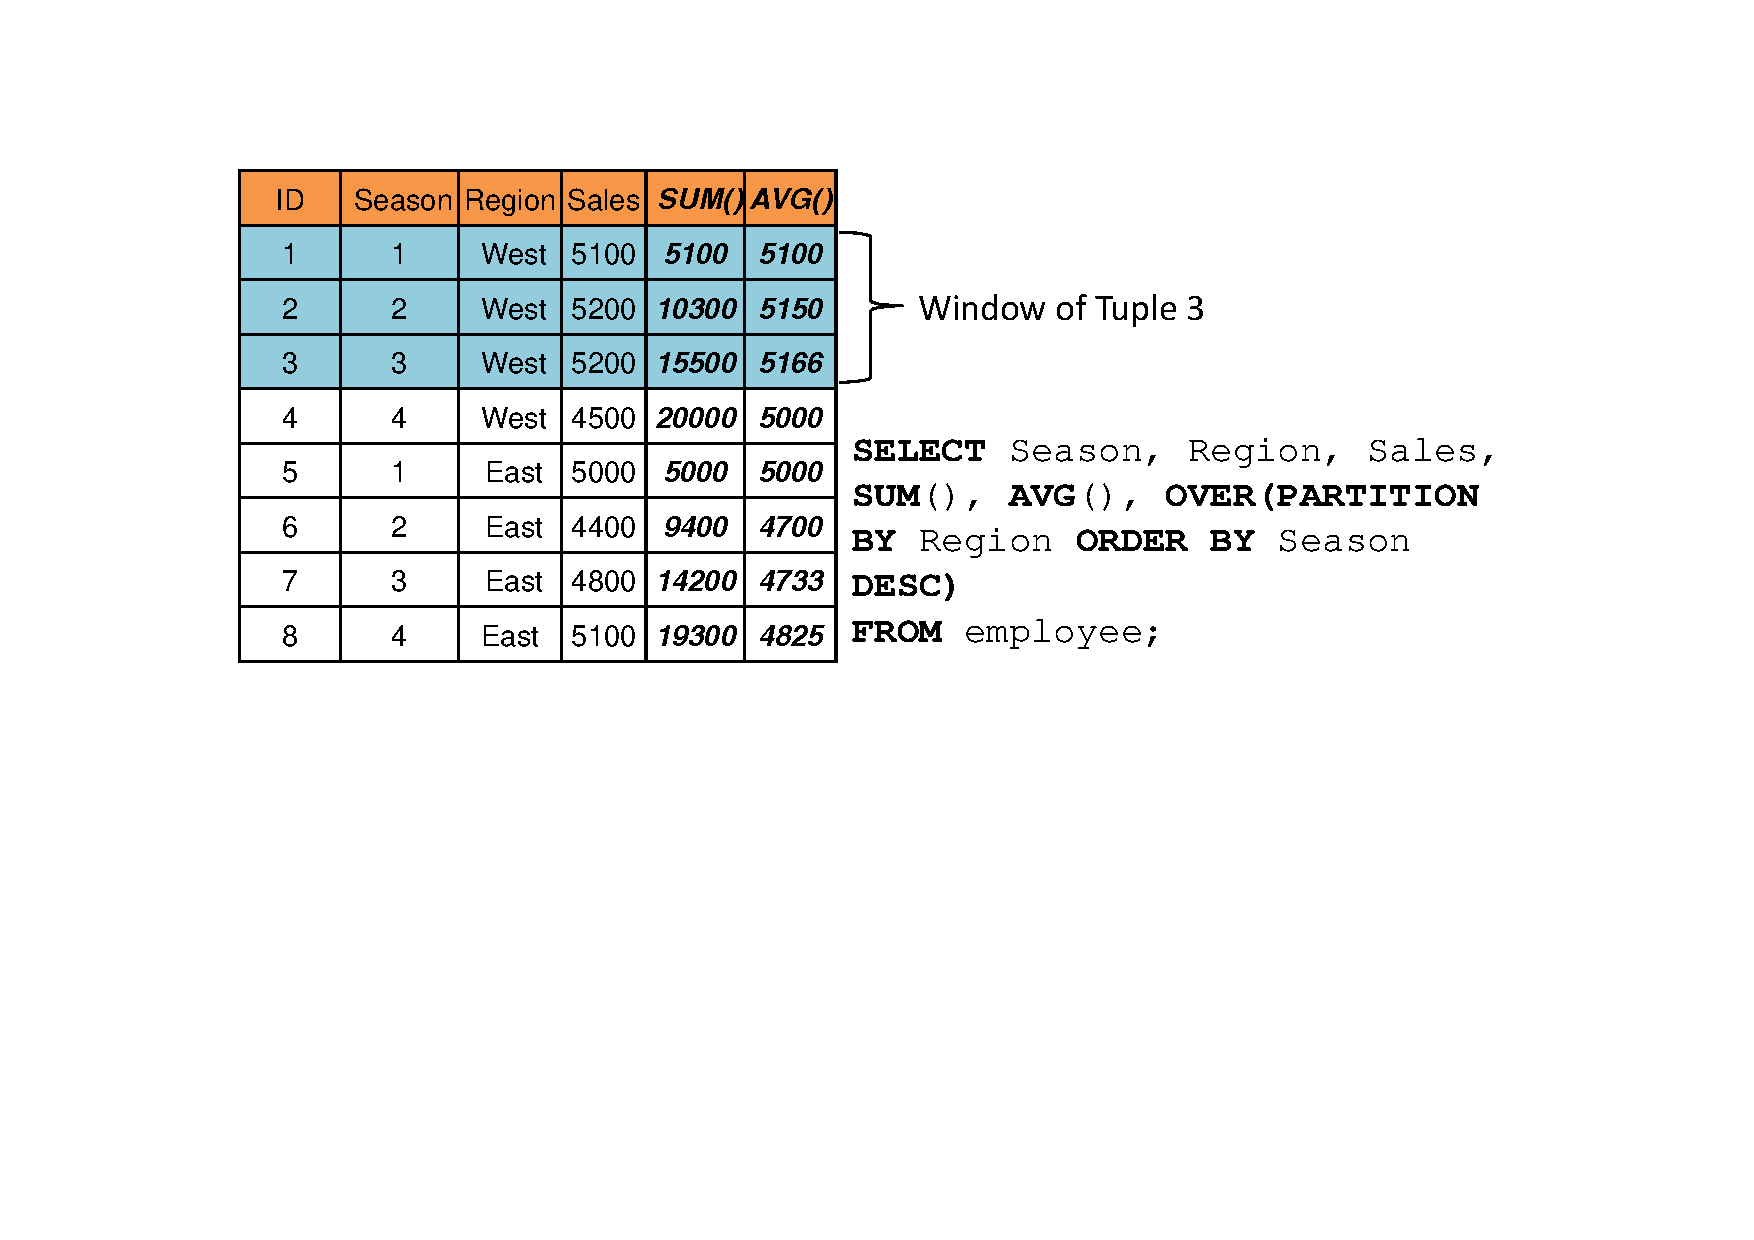
\includegraphics[width=0.8\linewidth]{window_example.pdf}
\caption{A SQL window function computing running sum and average of
sales. The window of season-3 is highlighted.} 
\label{fig:window}
\end{figure}

As shown in the figure, the sales report contains five attributes: 
``Season'', ``Region'' and ``Sales'' are the original fields, ``$\mathtt{sum()}$'' and ``$\mathtt{avg()}$''
are the analytics representing the running sum and average. A window function
is represented by the $\mathtt{over}$ keyword. In this context, the window of a tuple $o_i$
contains other tuples $o_j$ such that $o_i$ and $o_j$ are in the same ``region'' and $o_j$'s ``season'' is
prior to $o_i$'s. The window of season-$3$ for region-``West'' is highlighted.

Apart from this example, there are many other 
usages of the window function in the relational context. 
Being aware of the success of the window function, 
SQL~11 standard incorporates ``$\mathtt{LEAD}$'' and ``$\mathtt{LAG}$'' 
keywords which offer fine-grained specifications on a tuple's window.

Despite the usefulness, there are few works reporting the window
analytics in the non-relational context. This may dues to the
usage of \emph{sorting} in relational windows. For example,
in Figure~\ref{fig:window},
objects needs to be sorted according to ``Season'', and then the windows of
each object are implicitly formed. However, 
in non-relational context, sorting may be ambiguous and even undefined.

To generalize the window function to other data domains, we define the neighborhood
analytics in a broader context. Given a set of objects 
(such as tuples in relational context or vertexes in graph context),
the neighborhood analytic is a composite function
$(\mathcal{F} \circ \mathcal{N})$ applied on every object. $\mathcal{N}$
is the \emph{neighborhood function}, which contains the related objects of $o$;
$\mathcal{F}$ is an \emph{analytic function}, which could be aggregate, rank,
pattern matching, etc.
%the neighborhood analytic instance consists of two parts: a neighborhood indicator
%function $\mathbb{N}(o_i,o_j)$ deciding whether $o_j$ is in $o_i$'s neighborhoods,
%and an analytic function $f$ which aggregates a set of objects.  
%Let $N(o_i)$ be
%the set of neighbors of $o_i$, the neighborhood analytic aims to compute $f(N(o_i))$
%for all objects.
Apparently, relational window functions is a special case of such defined 
neighborhood analytics. For example, window function in Figure~\ref{fig:window} 
can be represented as $\mathcal{N}(o_i)=\{o_j | o_i.season > o_j.season \wedge o_i.region = o_j.region\}$
and $\mathcal{F} = \mathtt{avg}$.
Since the \emph{sorting} requirement is relaxed, our definition of neighborhood analytics
enriches the semantic of relational window notations 
and can be applied on other domains.
%
%Intuitively, we enrich the semantic of neighborhood as compared to the relation
%window notations. And our definition directly supports relational window notations by setting $\mathcal{N}$
%to capture the $\mathtt{over}$ clause. Since the \emph{sorting} is not required, such a 
%
%
%and is able to be
%applied on other data domains.


\section{Scope of the thesis}
In this thesis, we explore the neighborhood analytics in
different data domains. Our efforts showcase the usefulness of the neighborhood
concepts in those data domains and address the efficiency issues when adopting
nontrivial analytics. In particular, we looked at three most prevalent data domains, namely \textbf{attributed graph},
\textbf{time series} and \textbf{moving objects}. 
We then categorize two intuitive neighborhood functions as follows:

\textbf{Distance Neighborhood}: the neighborhood is defined based on numeric distance, that is $\mathcal{N}(o_i,K) = \{o_j | \mathtt{dist}(o_i,o_j) \leq K \}$, where $\mathtt{dist}$ is a distance function and $K$ is a distance threshold.

\textbf{Comparison Neighborhood}: the neighborhood is defined based on the comparison of objects, that is $\mathcal{N}(o) = \{o_i | o.a_m \ \mathtt{cmp} \ o_i.a_m\}$, where $a_m$ is an attribute of object
and $\mathtt{cmp}$ is a binary comparator.

There could be other types of neighborhoods with more fine-grained or more general definitions. In this thesis, we demonstrate
that these two simple neighborhood definitions
together with traditional analytic functions are already versatile in generating many useful analytics in various data domains.

\section{Contributions}
At a high level, this thesis entitles a bi-folded contribution.
First, by
sewing different $\mathcal{N}$s and $\mathcal{F}$s, three interesting
neighborhood analytic queries are proposed for \emph{graph}, \emph{trajectory}
and \emph{time series} domains respectively. Second, this thesis
deals with the technical issues in efficiently deploying corresponding analytic queries to
handle data in nowadays scale.
The road map of this thesis is as show in Figure~\ref{fig:thesis_roadmap}.
\begin{figure}[h]
\centering
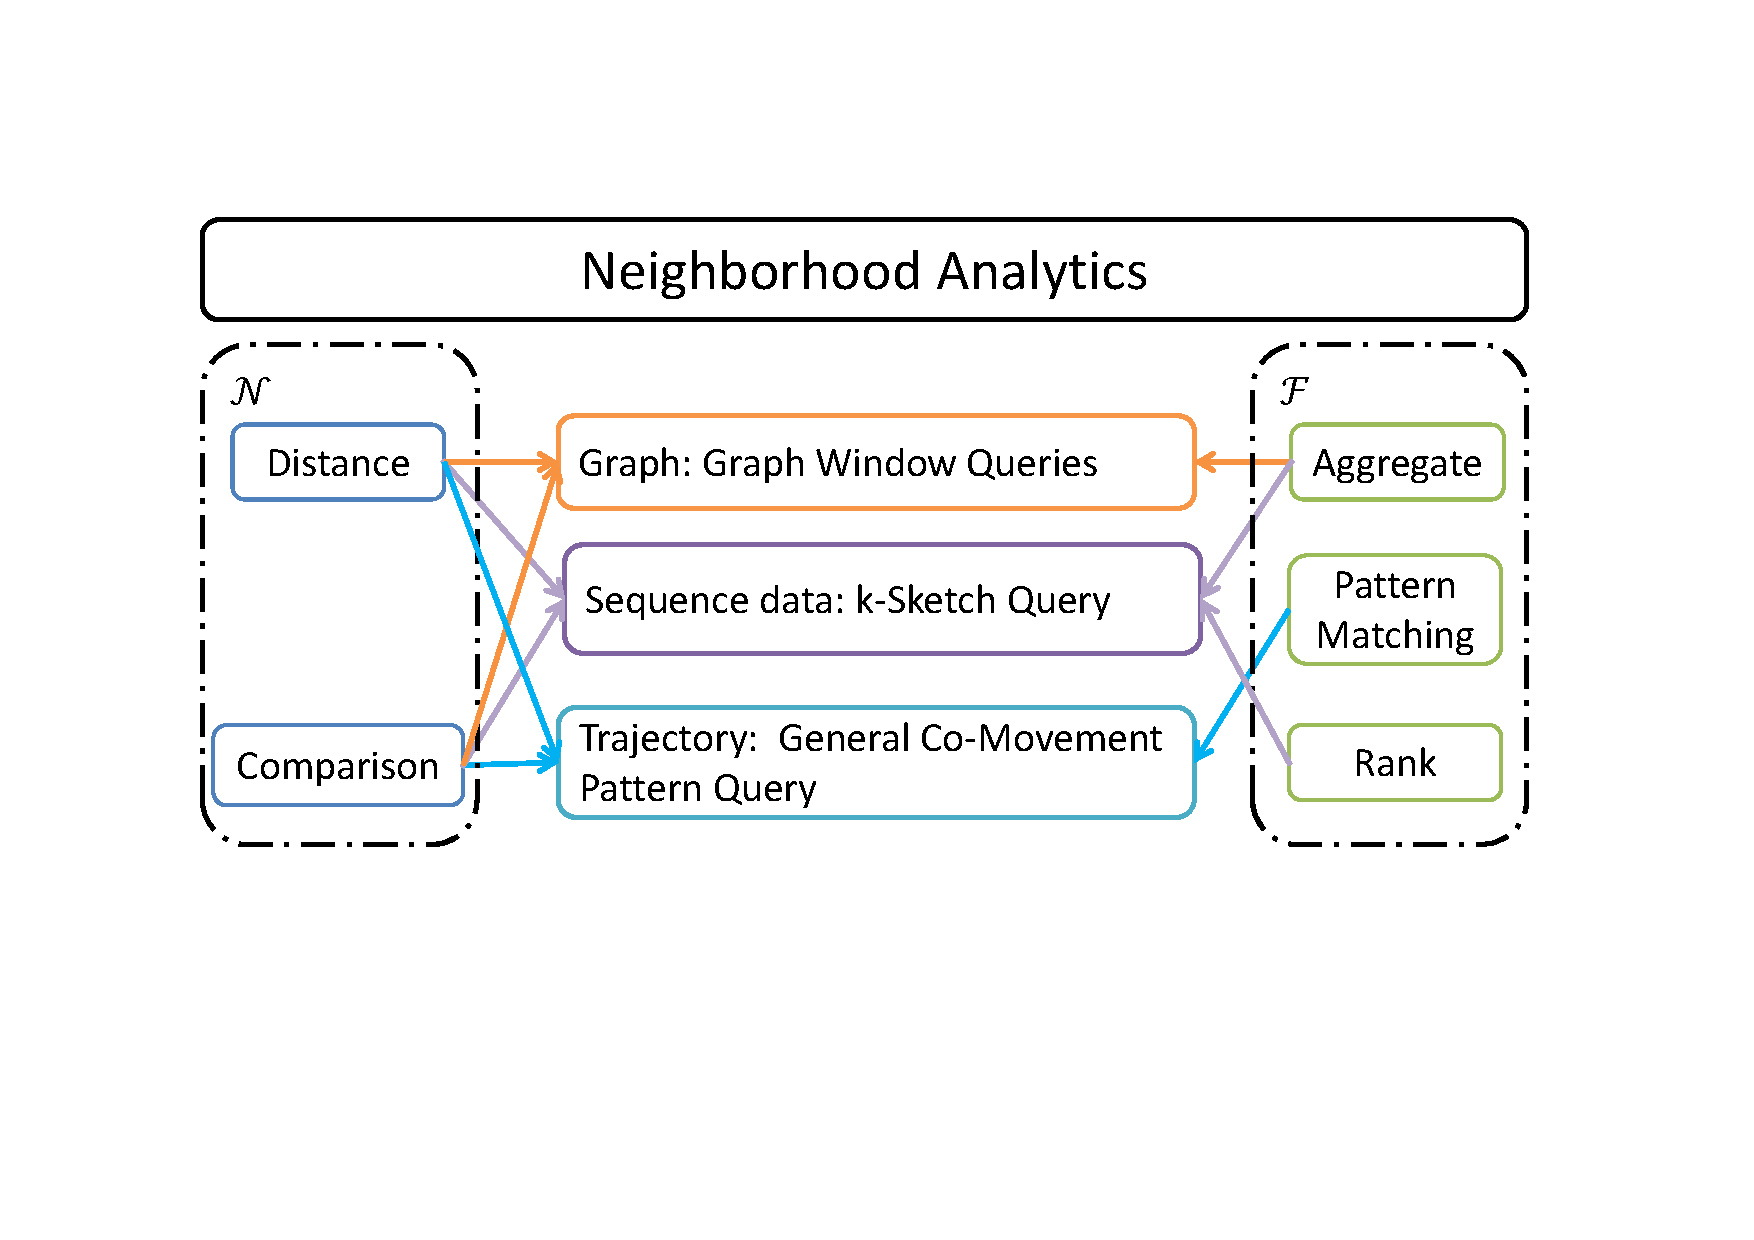
\includegraphics[width=0.8\linewidth]{thesis_roadmap.pdf}
\caption{The road map of this thesis. There are three major contributions as highlighted in the center. Each contribution
is a neighborhood analytic based on different $\mathcal{N}$ and $\mathcal{F}$ as indicated by arrows.} 
\label{fig:thesis_roadmap}
\end{figure}

\subsection{Graph Window Analytics}
This first piece of the thesis deals with neighborhood analytics
on graphs. Nowadays information network are typically
modeled as attributed graphs where the 
vertexes correspond to objects and the edges capture the
relationships between these objects. As vertexes embed a wealth
of information (e.g., user profiles in social networks), there are 
emerging demands on analyzing these data to extract useful insights. We propose the concept of \emph{window query} in the attributed graph context and identify two types of such queries as shown in the following examples:

\begin{example}[$k$-hop window]
In a social network (such as Linked-In and Facebook etc.), users are normally modeled as vertexes and connectivity relationships are modeled as edges. In social network scenario, it is of great interest to summarize the most relevant connections to each user such as the neighbors within $2$-hops. Some analytic queries such as summarizing the related connections' distribution among different companies, and computing age distribution of the related friends can be useful. In order to answer these queries, collecting data from every user's neighborhoods within 2-hop is necessary.
\end{example}
\begin{example}[Topological window]
In biological networks (such as Argocyc, Ecocyc etc.), genes, enzymes and proteins are vertexes and their
dependencies in a pathway are edges. Because these networks are directed and acyclic, 
in order to study the protein regulating process, one may be interested to find out the statistics of molecules in each protein production pathway. For each protein,we can traverse the graph to find every other 
 molecule that is in the upstream of its pathway. Then we can group and 
 count the number of genes and enzymes among those molecules.
\end{example}

The two \emph{windows} shown in the examples are essentially neighborhood functions defined for each vertex. Specifically, let $G=(V:E:A)$ be an attribute graph, where $V$ is the set of vertexes, $E$ is the set of edges, and each vertex $v$ is associated as a multidimensional points $a_v \in A$.
The \emph{k-hop} window is a \emph{distance} neighborhood function, 
i.e., $\mathcal{N}_k(v)= \{u|\mathtt{dist}(v,u) \leq K\}$, 
which captures the vertexes that are $k$-hop nearby. 
The \emph{topological} window,  $\mathcal{N}_t(v)= \{u | u \in v.ancestor\}$,
is a \emph{comparison} neighborhood function that captures
the ancestors of a vertex in a directly acyclic graph.  The analytic function $\mathcal{F}$ is an aggregate function (sum, avg, etc.) on $A$.

Apart from demonstrating the useful use-cases on these two windows, we also strive to support efficient window processing. We propose
two different types of indexes: Dense Block Index (DBIndex)
and Inheritance Index (I-Index). The DBIndex and I-Index
are specially optimized to support k-hop window and topological
window query processing. We develop the indexes
by integrating the window aggregation sharing techniques
to salvage partial work done for efficient computation. 
In addition, we develop space and performance efficient techniques
for index construction. In our experiments, DBIndex saves upto 80\%
of indexing time as compared to the state-of-the-art competitor.


\subsection{Automatic News Discovery in Time Series Data}
The second piece of the thesis proposes a neighborhood
query on automatic discovery of news in the time series data.
Nowadays events are collected in a timestamped format and journalists needs to manually synthesize those events to write interesting news. We propose the automatic \emph{rank-aware news theme} detection with the aim to relieve journalists from manually poring over a large amount of data. Particularly, we strive to
automatically detect the following news themes that are prevalent in real life news reports: 

\begin{enumerate}
\setlength\itemsep{-0.05cm}
\item(Feb 26, 2003) With 32 points, Kobe Bryant saw his 40+ scoring streak end at \textbf{nine} games,  tied with Michael Jordan for \textbf{fourth} place on the all-time list\footnote{\url{http://www.nba.com/features/kobe_40plus_030221.html}}. 

\item(April 14, 2014) Stephen Curry has made 602 3-pointer attempts from beyond the arc,... are the \textbf{10th} most in NBA history in a season (\textbf{82 games})\footnote{\url{http://www.cbssports.com/nba/eye-on-basketball/24525914/stephen-curry-makes-history-with-consecutive-seasons-of-250-3s}}.

\item (May 28, 2015) Stocks gained for the \textbf{seventh consecutive day} on Wednesday as the benchmark moved close to the 5,000 mark for \textbf{the first} time in seven years\footnote{\url{http://www.zacks.com/stock/news/176469/china-stock-roundup-ctrip-buys-elong-stake-trina-solar-beats-estimates}}.

\item (Jun 9,  2014) Delhi has been witnessing a spell of hot weather  over the \textbf{past month}, with temperature hovering around 45 degrees Celsius, .... \textbf{highest} ever since 1952\footnote{\url{http://www.dnaindia.com/delhi/report-delhi-records-highest-temperature-in-62-years-1994332}}.

\item(Jul 22, 2011) Pelican Point recorded a maximum rainfall of 0.32 inches for \textbf{12 months}, making it the  \textbf{9th driest} places on earth\footnote{\url{http://www.livescience.com/30627-10-driest-places-on-earth.html}}.
\end{enumerate}


In the above news themes, there are a subject (e.g., Kobe Bryant, Stocks, Delhi), an event window (e.g., nine straight games, seventh consecutive days, past month), an aggregate function on an attribute
(e.g., minimum points, count of gains, average of degrees), a rank (e.g., fourth, first time, highest), and a
historical dataset (e.g., all time list, seven years, since 1952). These news theme indicators are summarized in Table~\ref{tbl:news-example}.  


\begin{table}[h]
\centering
\begin{tabular}{|c|c|c|c|}
\hline
\textbf{E.g.} & \textbf{Aggregate function} & \textbf{Event window} & \textbf{Rank} \\
\hline
1 & min(points) & 9 straight games & 4 \\
\hline
2 & sum(shot attempts) & 82 games & 10 \\
%$\frac{\text{sum}(\cdot, \text{goal})}{\text{sum}(\cdot, \text{goal})+\text{sum}(\cdot, \text{miss})}$ & five game winning streak & 2
\hline
%2 & min($\cdot$, contracts) & 4 straight months & 1 \\
%\hline
3 & count(gains) & 7 consecutive days & 1 \\
\hline
4 & average(degree) & past months (30 days) & 1 \\
\hline
5 & max(raindrops) & 12 months & 9 \\
\hline
\end{tabular}
\caption{News theme summary}
\label{tbl:news-example}
\end{table}


We model these news themes using nested neighborhood analytics. Let $e_s(t)$ denote the event of subject $s$ at time $t$. Then the news themes are generated in a two-step manner: 

(1) a \emph{distance neighborhood} $\mathcal{N}_1(o_i,w)=\{o_j | o_i.t - o_j.t \leq w \}$ groups a consecutive $w$ events for each event. Let $\overline{v}$ be the aggregate value associated with $\mathcal{N}_1$, then the output of this step is a set of \emph{event windows} of the form  $\langle o_i, w, t, \overline{v} \rangle$.

(2) a \emph{comparison neighborhood} $\mathcal{N}_2(o_i) = \{o_j | o_j.w = o_i.w \wedge o_i.\overline{v} \geq o_j.\overline{v} \}$ ranks a subject's event window among all other event windows with the same window size. The result of the this step is a tuple $\langle o_i, w, t, r \rangle$, where $r$ is the \emph{rank}.

The resulting news themes from $\mathcal{N}_2 \cdot \mathcal{N}_1$ is referred as \emph{rank-aware news themes}. Rooted from the useful \emph{rank-aware news themes}, we further propose
a novel concept named \emph{Sketch} to avoid outputting near-duplicate themes.
A sketch contains $k$ most representative rank-aware news themes under a scoring function that considers both strikingness and diversity.  Our objective is to discover sketches for each subject in the domain.

We study the problem in both
offline and online scenarios, and propose various window-level 
pruning techniques to find striking candidate themes.
Among those candidates, we then develop approximation
methods, with theoretical bounds, to discover the $k$ most
representative themes. We conduct experiments on four real
datasets, and the results demonstrate the efficiency and 
effectiveness of our proposed algorithms: the running time
achieves up to 500 times speedup and the quality of the
detected news themes is endorsed by the anonymous users
from Amazon Mechanical Turk \footnote{\url{https://requester.mturk.com}}.

\subsection{Mining Co-Movement Patterns in Trajectory Databases}
The third piece of the thesis addresses the neighborhood
query on trajectories.
Discovering co-movement patterns from large-scale trajectory 
databases is an important mining task and has a wide
spectrum of applications. 
Existing studies have identified several types of interesting co-movement patterns called \emph{co-movement} pattern. A co-movement pattern refers to a group of moving objects traveling together for a certain period of time and the group of objects is normally determined by their spatial proximity. A pattern is prominent if the group size exceeds $M$ and the length of duration exceeds $K$. 
Rooted from such a basic definition 
and driven by different mining applications, there are a bunch of variants 
of co-movement patterns that have been developed with more advanced constraints.

\begin{figure}[h]
\centering
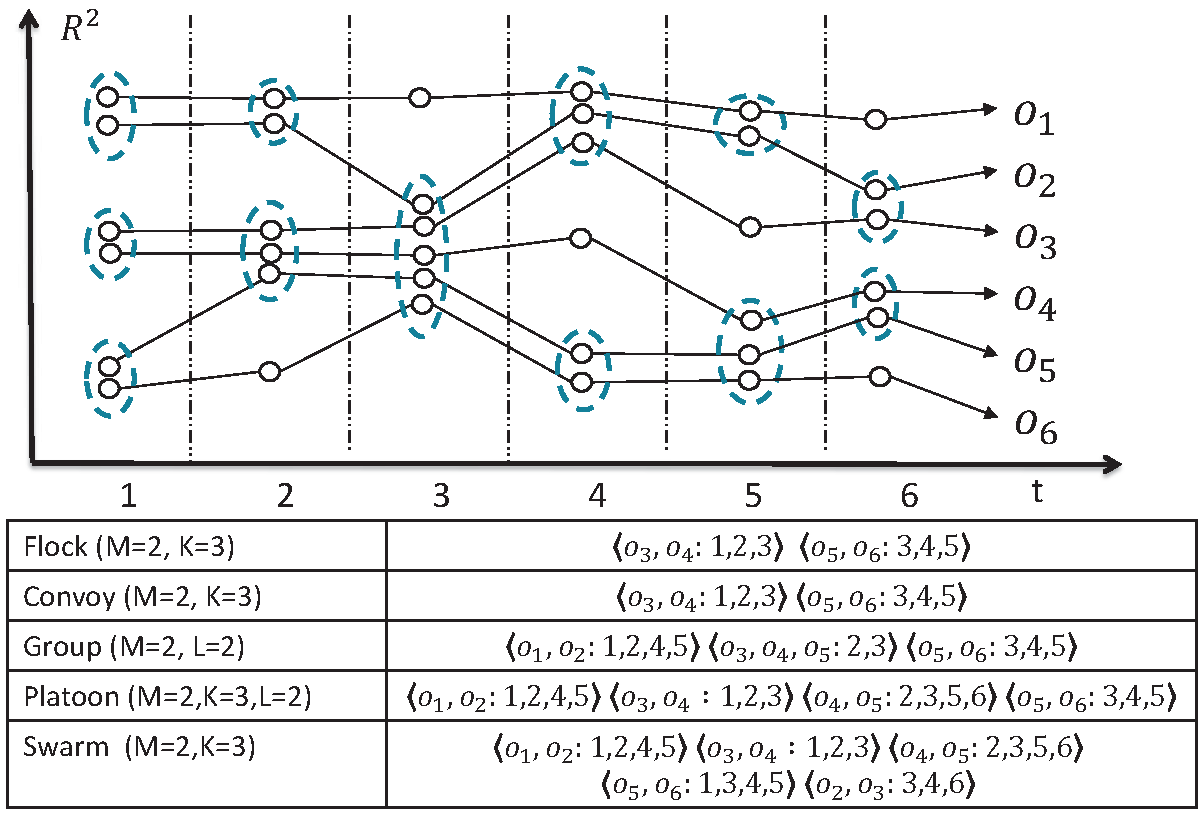
\includegraphics[width=0.8\textwidth]{trajectory_patterns.pdf}
\caption{Trajectories and co-movement patterns. The example consists of six trajectories across six snapshots. Objects in spatial clusters are enclosed by dotted circles. $M$ is the minimum cluster cardinality; $K$ denotes the minimum number of snapshots for the occurrence of a spatial cluster; and $L$ denotes the minimum length for local consecutiveness.}
\label{fig:related_work}
\end{figure}

Figure~\ref{fig:related_work} is an example to demonstrate the concepts of various co-movement patterns. The trajectory database consists of six moving objects and the temporal dimension is discretized into six snapshots. In each snapshot, we treat the clustering method as a black-box and assume that they generate the same clusters. Objects in proximity are grouped in the dotted circles. As aforementioned, there are three parameters to determine the co-movement patterns and the default settings in this example are $M=2$, $K=3$ and $L=2$. Both the \emph{flock} and the \emph{convoy} require the spatial clusters to last for at least $K$ consecutive  timestamps. Hence,$\langle o_3,o_4:1,2,3 \rangle$ and $\langle o_5,o_6:3,4,5 \rangle$  remains the only two candidates matching the patterns. The \textit{swarm} relaxes the pattern matching by discarding the temporal consecutiveness constraint. Thus, it generates many more candidates than the \textit{flock} and the \textit{convoy}. The \textit{group} and the \textit{platoon} add another constraint on local consecutiveness to retain meaningful patterns. For instance, $\langle o_1,o_2:1,2,4,5 \rangle$ is a pattern matching local consecutiveness because timestamps $(1,2)$ and $(4,5)$ are two segments with length no smaller than $L=2$. The difference between the \textit{group} and the \textit{platoon} is that the \textit{platoon} has an additional parameter $K$ to specify the minimum number of snapshots for the spatial clusters. This explains why $\langle o_3,o_4,o_5:2,3 \rangle$ is a \textit{group} pattern but not a \textit{platoon} pattern.



We notice that these patterns can be unified using \emph{neighborhood} query. Let $C_t(o_i)$ be the cluster $o_i$ belongs to at snapshot $t$, then a co-movement pattern 
can be viewed as a \emph{comparison neighborhood} $\mathcal{N}(o_i)=\{o_j, T | \exists t \in T, C_t(o_i) = C_t(o_j)\}$. For each generated neighborhood, the analytic function is the pattern discovery
based on temporal constraints. We then propose a \emph{General Co-Movement Pattern} (GCMP) based on the neighborhood to capture all existing co-movement patterns. The GCMP can be reduced to any of the existing co-movement patterns by applying on with different analytic functions.

Technical wise, we study efficiently processing GCMP in a MapReduce platform to gain scalability for large-scale trajectories. We propose two parallel frameworks: (1) TRPM partition trajectories by replicating snapshots in the temporal domain, within each partition, a line-sweep method is developed to find all patterns. (2) SPARE partition trajectories based on object's neighborhood. Within each partition, a variant of Apriori enumerator is applied to generate all patterns. We then show the efficiency of both our methods in Apache Spark platforms with three real trajectory datasets upto 170 million points. The results show that SPARE achieves upto 14 times efficiency as compared to TRPM, and 112 times speedup as compared to the state-of-the-art centralized schemes.

\section{Thesis Organization}
The remaining part of the thesis are organized as follows: in Chapter 2, we summarize related literature on neighborhood related analytics in different data domains. In Chapter 3, we present the window function on graph data. In Chapter 4, we present a news discovery application on time series data.
In Chapter 5, we present a pattern mining framework on trajectory data. Chapter 6 summarizes this thesis and highlights the future directions.